\chapter{Experiments}
In this section, we present our findings.
We expect that our algorithm will improve the training process for a regular deep learning user, both in the perspective of training performance and in final accuracy.
This hypothesis is borne out in the smaller datasets, but remains somewhat inconclusive for larger datasets.
Nevertheless, we note that there are significant points of interest that are raised as a result, and the potential for improvement on this algorithm is encouraging.

\section{Function Regression}
Our first experiment is relatively simplistic, but is also indicative of the basic algorithm's performance.
In this experiment, we approximate the trigonometric sine function in the range of $[-2\pi, 2\pi]$.
Our architecture for this experiment is extremely simple: it is merely a feedforward network with one hidden layer consisting of up to 500 nodes.
This is sufficient capacity to learn the sine function with great accuracy, but can still be heavily affected by the training regime applied to it.
We investigate the importance of the hidden layer's capacity by testing static networks of 100 and 500 nodes, then compare these results to a dynamically sizing network.

For this experiment, we split the network into fifths, and initialize them all before any training begins.
We initially only let the network use the first fifth of its capacity, making it equivalent to the 100-node static test.
We track the moving average of the error, and after it fails to rise within the last 10 batches, we proceed to increase the capacity of the network by a fifth, but also freeze the existing capacity.
This serves to force the additional capacity to learn the mistakes of the existing capacity, rather than just adding additional parameters that would change alongside the original.
We see the results of the experiment in Figure~\ref{fig:sin_loss}, in which our method is labelled ``adaptive.''

\begin{figure}[!htb]
\centering
\resizebox{0.8\textwidth}{!}{% GNUPLOT: LaTeX picture with Postscript
\begingroup
  \makeatletter
  \providecommand\color[2][]{%
    \GenericError{(gnuplot) \space\space\space\@spaces}{%
      Package color not loaded in conjunction with
      terminal option `colourtext'%
    }{See the gnuplot documentation for explanation.%
    }{Either use 'blacktext' in gnuplot or load the package
      color.sty in LaTeX.}%
    \renewcommand\color[2][]{}%
  }%
  \providecommand\includegraphics[2][]{%
    \GenericError{(gnuplot) \space\space\space\@spaces}{%
      Package graphicx or graphics not loaded%
    }{See the gnuplot documentation for explanation.%
    }{The gnuplot epslatex terminal needs graphicx.sty or graphics.sty.}%
    \renewcommand\includegraphics[2][]{}%
  }%
  \providecommand\rotatebox[2]{#2}%
  \@ifundefined{ifGPcolor}{%
    \newif\ifGPcolor
    \GPcolorfalse
  }{}%
  \@ifundefined{ifGPblacktext}{%
    \newif\ifGPblacktext
    \GPblacktexttrue
  }{}%
  % define a \g@addto@macro without @ in the name:
  \let\gplgaddtomacro\g@addto@macro
  % define empty templates for all commands taking text:
  \gdef\gplbacktext{}%
  \gdef\gplfronttext{}%
  \makeatother
  \ifGPblacktext
    % no textcolor at all
    \def\colorrgb#1{}%
    \def\colorgray#1{}%
  \else
    % gray or color?
    \ifGPcolor
      \def\colorrgb#1{\color[rgb]{#1}}%
      \def\colorgray#1{\color[gray]{#1}}%
      \expandafter\def\csname LTw\endcsname{\color{white}}%
      \expandafter\def\csname LTb\endcsname{\color{black}}%
      \expandafter\def\csname LTa\endcsname{\color{black}}%
      \expandafter\def\csname LT0\endcsname{\color[rgb]{1,0,0}}%
      \expandafter\def\csname LT1\endcsname{\color[rgb]{0,1,0}}%
      \expandafter\def\csname LT2\endcsname{\color[rgb]{0,0,1}}%
      \expandafter\def\csname LT3\endcsname{\color[rgb]{1,0,1}}%
      \expandafter\def\csname LT4\endcsname{\color[rgb]{0,1,1}}%
      \expandafter\def\csname LT5\endcsname{\color[rgb]{1,1,0}}%
      \expandafter\def\csname LT6\endcsname{\color[rgb]{0,0,0}}%
      \expandafter\def\csname LT7\endcsname{\color[rgb]{1,0.3,0}}%
      \expandafter\def\csname LT8\endcsname{\color[rgb]{0.5,0.5,0.5}}%
    \else
      % gray
      \def\colorrgb#1{\color{black}}%
      \def\colorgray#1{\color[gray]{#1}}%
      \expandafter\def\csname LTw\endcsname{\color{white}}%
      \expandafter\def\csname LTb\endcsname{\color{black}}%
      \expandafter\def\csname LTa\endcsname{\color{black}}%
      \expandafter\def\csname LT0\endcsname{\color{black}}%
      \expandafter\def\csname LT1\endcsname{\color{black}}%
      \expandafter\def\csname LT2\endcsname{\color{black}}%
      \expandafter\def\csname LT3\endcsname{\color{black}}%
      \expandafter\def\csname LT4\endcsname{\color{black}}%
      \expandafter\def\csname LT5\endcsname{\color{black}}%
      \expandafter\def\csname LT6\endcsname{\color{black}}%
      \expandafter\def\csname LT7\endcsname{\color{black}}%
      \expandafter\def\csname LT8\endcsname{\color{black}}%
    \fi
  \fi
    \setlength{\unitlength}{0.0500bp}%
    \ifx\gptboxheight\undefined%
      \newlength{\gptboxheight}%
      \newlength{\gptboxwidth}%
      \newsavebox{\gptboxtext}%
    \fi%
    \setlength{\fboxrule}{0.5pt}%
    \setlength{\fboxsep}{1pt}%
\begin{picture}(7200.00,5040.00)%
    \gplgaddtomacro\gplbacktext{%
      \csname LTb\endcsname%
      \put(1210,1374){\makebox(0,0)[r]{\strut{}$0.0001$}}%
      \put(1210,1829){\makebox(0,0)[r]{\strut{}$0.001$}}%
      \put(1210,2284){\makebox(0,0)[r]{\strut{}$0.01$}}%
      \put(1210,2740){\makebox(0,0)[r]{\strut{}$0.1$}}%
      \put(1210,3195){\makebox(0,0)[r]{\strut{}$1$}}%
      \put(1210,3650){\makebox(0,0)[r]{\strut{}$10$}}%
      \put(1210,4105){\makebox(0,0)[r]{\strut{}$100$}}%
      \put(1342,1154){\makebox(0,0){\strut{}$0$}}%
      \put(1888,1154){\makebox(0,0){\strut{}$10$}}%
      \put(2434,1154){\makebox(0,0){\strut{}$20$}}%
      \put(2980,1154){\makebox(0,0){\strut{}$30$}}%
      \put(3526,1154){\makebox(0,0){\strut{}$40$}}%
      \put(4073,1154){\makebox(0,0){\strut{}$50$}}%
      \put(4619,1154){\makebox(0,0){\strut{}$60$}}%
      \put(5165,1154){\makebox(0,0){\strut{}$70$}}%
      \put(5711,1154){\makebox(0,0){\strut{}$80$}}%
      \put(6257,1154){\makebox(0,0){\strut{}$90$}}%
      \put(6803,1154){\makebox(0,0){\strut{}$100$}}%
    }%
    \gplgaddtomacro\gplfronttext{%
      \csname LTb\endcsname%
      \put(176,2739){\rotatebox{-270}{\makebox(0,0){\strut{}log loss}}}%
      \put(4072,824){\makebox(0,0){\strut{}epoch}}%
      \csname LTb\endcsname%
      \put(5816,3932){\makebox(0,0)[r]{\strut{}100-node static}}%
      \csname LTb\endcsname%
      \put(5816,3712){\makebox(0,0)[r]{\strut{}500-node static}}%
      \csname LTb\endcsname%
      \put(5816,3492){\makebox(0,0)[r]{\strut{}adaptive}}%
    }%
    \gplbacktext
    \put(0,0){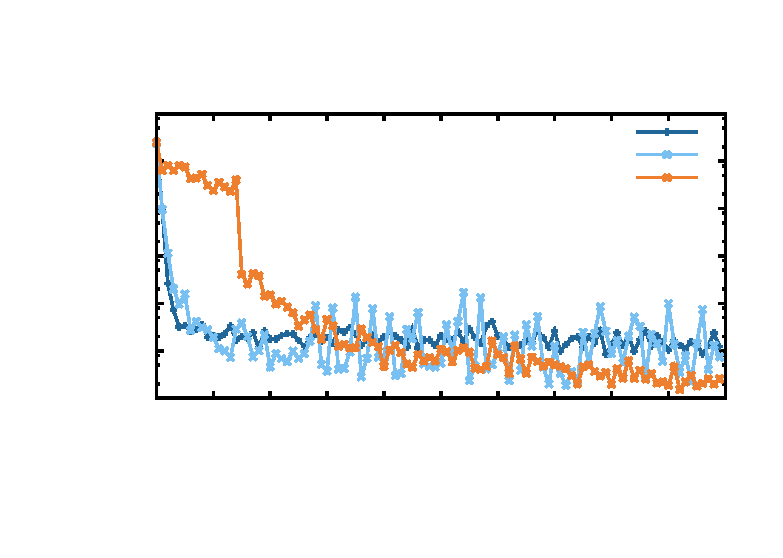
\includegraphics{sin}}%
    \gplfronttext
  \end{picture}%
\endgroup
}
\caption{Sine function approximation by different methods.}
\label{fig:sin_loss}
\end{figure}

It is immediately clear that our method is able to converge to a much better solution than simple training methods.
Importantly, we plot the y-axis on the logarithmic scale, so small improvements are in fact extremely significant.
Firstly, we note that increasing the capacity of the network from 100 to 500 nodes does not have a significant impact on final error.
In fact, the 500-node result would generally be considered worse, as it exhibits far noisier behavior.
On quick inspection, the adaptive method is generally superior in every way.
Surprisingly, however, the adaptive network is initially slower to train compared to the 100-node network, despite utilizing same capacity. 
We suspect this difference has to do with the potential variances in optimizer and initializer performance discussed above.
Regardless of its early-stage performance, we can see that it benefits tremendously from increased capacity, and overtakes the both of the static networks by around epoch 35.
There are some small spikes in error which we attribute to the sudden increase in capacity, but overall the performance is consistently better than that of the static methods.

\begin{table}[!htb]
\centering
\caption{Final-10 errors for various methods.}
\label{table:sin_errors}
\begin{tabular}{@{}lrr@{}}
\toprule
Network  & Mean    & Standard Deviation \\ \midrule
100-node & 0.00138 & 0.000389           \\
500-node & 0.00234 & 0.003261           \\
Adaptive & 0.00024 & 0.000084           \\ \bottomrule
\end{tabular}
\end{table}

To measure these results quantitatively, we consider both the average and the standard deviations of loss over the final 10 samples.
These results are presented in Table~\ref{table:sin_errors}.
We can see that the noisier results of the 500-node network are actually noticeably worse when averaged---it has nearly twice the error of the smaller 100-node network.
Furthermore, the standard deviation is an order of magnitude larger over the 100-node network., which is extremely poor as it is larger than the average error.
In contrast, the adaptive method exhibits both lower mean and standard deviation in the long run.
This indicates an improvement not just in learning capacity, but also in stability, which is a crucial property for training as noisy behavior is indicative of a number of other problems.
Chief amongst these is the simple problem that noisy behavior makes it difficult to decide when an experiment has concluded.
In any case, throughout this experiment, the adaptive method has offered significant improvements in performance over either static network.

\section{MNIST Classifier}
Modern deep learning algorithms have generally tended to be developed for image classification purposes, in part due to the original usage of convolutional neural networks.
LeCun et al.'s original work with CNNs \cite{lecun1998gradient} was in designing a classifier for the MNIST dataset, a collection of monochrome handwritten digits.
These images have been preprocessed for regularity, and have all been resized to a standard $28\times 28$ resolution.
MNIST is a well-regarded small image classification dataset which serves as a useful benchmark for this algorithm.


Tensorflow includes MNIST support as part of the base installation as part of its example code, so we are able to rely on a simple interface to download, load, and process the image data according to standard image augmentation purposes.
For the purposes of this experiment, we follow the example convolutional neural network provided by Google \cite{deepmnist}, and modify it so we can apply our expansion algorithm.
This is a typical structure, with two convolutional layers utilizing $7\times 7$ kernels, and then a fully-connected layer of 1024 nodes.
While this is far from the best known architectures for MNIST, it serves as a good baseline and is easily accessible.
Once again, we apply our methodology of training the network in portions.
This time, due to the increased capacity of the network, we instead train it in tenths, once again expanding when the moving average of accuracy begins to stall or decrease.

\begin{figure}[!htb]
\centering
\resizebox{0.8\textwidth}{!}{% GNUPLOT: LaTeX picture with Postscript
\begingroup
  \makeatletter
  \providecommand\color[2][]{%
    \GenericError{(gnuplot) \space\space\space\@spaces}{%
      Package color not loaded in conjunction with
      terminal option `colourtext'%
    }{See the gnuplot documentation for explanation.%
    }{Either use 'blacktext' in gnuplot or load the package
      color.sty in LaTeX.}%
    \renewcommand\color[2][]{}%
  }%
  \providecommand\includegraphics[2][]{%
    \GenericError{(gnuplot) \space\space\space\@spaces}{%
      Package graphicx or graphics not loaded%
    }{See the gnuplot documentation for explanation.%
    }{The gnuplot epslatex terminal needs graphicx.sty or graphics.sty.}%
    \renewcommand\includegraphics[2][]{}%
  }%
  \providecommand\rotatebox[2]{#2}%
  \@ifundefined{ifGPcolor}{%
    \newif\ifGPcolor
    \GPcolorfalse
  }{}%
  \@ifundefined{ifGPblacktext}{%
    \newif\ifGPblacktext
    \GPblacktexttrue
  }{}%
  % define a \g@addto@macro without @ in the name:
  \let\gplgaddtomacro\g@addto@macro
  % define empty templates for all commands taking text:
  \gdef\gplbacktext{}%
  \gdef\gplfronttext{}%
  \makeatother
  \ifGPblacktext
    % no textcolor at all
    \def\colorrgb#1{}%
    \def\colorgray#1{}%
  \else
    % gray or color?
    \ifGPcolor
      \def\colorrgb#1{\color[rgb]{#1}}%
      \def\colorgray#1{\color[gray]{#1}}%
      \expandafter\def\csname LTw\endcsname{\color{white}}%
      \expandafter\def\csname LTb\endcsname{\color{black}}%
      \expandafter\def\csname LTa\endcsname{\color{black}}%
      \expandafter\def\csname LT0\endcsname{\color[rgb]{1,0,0}}%
      \expandafter\def\csname LT1\endcsname{\color[rgb]{0,1,0}}%
      \expandafter\def\csname LT2\endcsname{\color[rgb]{0,0,1}}%
      \expandafter\def\csname LT3\endcsname{\color[rgb]{1,0,1}}%
      \expandafter\def\csname LT4\endcsname{\color[rgb]{0,1,1}}%
      \expandafter\def\csname LT5\endcsname{\color[rgb]{1,1,0}}%
      \expandafter\def\csname LT6\endcsname{\color[rgb]{0,0,0}}%
      \expandafter\def\csname LT7\endcsname{\color[rgb]{1,0.3,0}}%
      \expandafter\def\csname LT8\endcsname{\color[rgb]{0.5,0.5,0.5}}%
    \else
      % gray
      \def\colorrgb#1{\color{black}}%
      \def\colorgray#1{\color[gray]{#1}}%
      \expandafter\def\csname LTw\endcsname{\color{white}}%
      \expandafter\def\csname LTb\endcsname{\color{black}}%
      \expandafter\def\csname LTa\endcsname{\color{black}}%
      \expandafter\def\csname LT0\endcsname{\color{black}}%
      \expandafter\def\csname LT1\endcsname{\color{black}}%
      \expandafter\def\csname LT2\endcsname{\color{black}}%
      \expandafter\def\csname LT3\endcsname{\color{black}}%
      \expandafter\def\csname LT4\endcsname{\color{black}}%
      \expandafter\def\csname LT5\endcsname{\color{black}}%
      \expandafter\def\csname LT6\endcsname{\color{black}}%
      \expandafter\def\csname LT7\endcsname{\color{black}}%
      \expandafter\def\csname LT8\endcsname{\color{black}}%
    \fi
  \fi
    \setlength{\unitlength}{0.0500bp}%
    \ifx\gptboxheight\undefined%
      \newlength{\gptboxheight}%
      \newlength{\gptboxwidth}%
      \newsavebox{\gptboxtext}%
    \fi%
    \setlength{\fboxrule}{0.5pt}%
    \setlength{\fboxsep}{1pt}%
\begin{picture}(7200.00,5040.00)%
    \gplgaddtomacro\gplbacktext{%
      \csname LTb\endcsname%
      \put(1078,1341){\makebox(0,0)[r]{\strut{}$0.001$}}%
      \put(1078,2273){\makebox(0,0)[r]{\strut{}$0.01$}}%
      \put(1078,3206){\makebox(0,0)[r]{\strut{}$0.1$}}%
      \put(1078,4138){\makebox(0,0)[r]{\strut{}$1$}}%
      \put(1210,1121){\makebox(0,0){\strut{}$0$}}%
      \put(1769,1121){\makebox(0,0){\strut{}$100$}}%
      \put(2329,1121){\makebox(0,0){\strut{}$200$}}%
      \put(2888,1121){\makebox(0,0){\strut{}$300$}}%
      \put(3447,1121){\makebox(0,0){\strut{}$400$}}%
      \put(4007,1121){\makebox(0,0){\strut{}$500$}}%
      \put(4566,1121){\makebox(0,0){\strut{}$600$}}%
      \put(5125,1121){\makebox(0,0){\strut{}$700$}}%
      \put(5684,1121){\makebox(0,0){\strut{}$800$}}%
      \put(6244,1121){\makebox(0,0){\strut{}$900$}}%
      \put(6803,1121){\makebox(0,0){\strut{}$1000$}}%
    }%
    \gplgaddtomacro\gplfronttext{%
      \csname LTb\endcsname%
      \put(176,2739){\rotatebox{-270}{\makebox(0,0){\strut{}log loss}}}%
      \put(4006,791){\makebox(0,0){\strut{}epoch}}%
      \csname LTb\endcsname%
      \put(5816,3965){\makebox(0,0)[r]{\strut{}adaptive}}%
      \csname LTb\endcsname%
      \put(5816,3745){\makebox(0,0)[r]{\strut{}standard}}%
    }%
    \gplbacktext
    \put(0,0){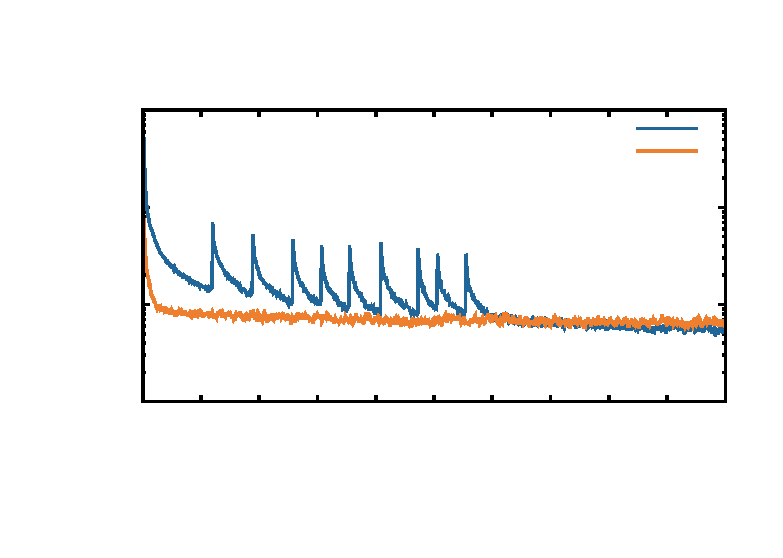
\includegraphics{mnist}}%
    \gplfronttext
  \end{picture}%
\endgroup
}
\caption{MNIST loss trained by different methods.}
\label{fig:mnist_loss}
\end{figure}

We show the results of the MNIST classifier in Figure~\ref{fig:mnist_loss}.
In this experiment, there are significant spikes to the loss when new capacity is added, indicating that the extra capacity produces a significant shock on the network.
We hypothesize that this is due to the fact that multiple layers are all increasing in capacity simultaneously, which leads to a much more pronounced change in outputs.
Whereas the previous experiment only involved a single layer, the interactions of additional units that are connected to the original network changes the dynamics significantly.
This still shows an improvement over the standard network, although the difference is much smaller than previously demonstrated.
This is likely due to the fact that the error is very low in both examples; typical algorithms achieve over 99\% accuracy on MNIST.
It appears that the adaptive network is still improving over time but may be limited by the length of the experiment, while the standard network has converged to its best potential.
We were not able to test this theory more fully due to time constraints, but leave it as a potential point of interest.
We also report the mean and standard deviation statistics for this experiment in Table~\ref{table:mnist_errors}. 
This corroborates the close performance between the two networks, but also demonstrates the improvements our adaptive method produces over a standard network of the same final size.
Both the error and the standard deviation are lower, indicating a mild improvement.

\begin{table}[!htb]
\centering
\caption{Comparison on MNIST.}
\label{table:mnist_errors}
\begin{tabular}{@{}lrr@{}}
\toprule
Network  & Mean    & Standard Deviation \\ \midrule
standard & 0.00686 & 0.000369           \\
adaptive & 0.00633 & 0.000248           \\ \bottomrule
\end{tabular}
\end{table}


\section{CIFAR-100}
One of the common modern image classification datasets is CIFAR-100, a set of 60000 images collected by researchers at the University of Toronto.
It consists of 20 classes, each with 5 subclasses.
For each of the 100 subclasses, there are 500 training images and 100 testing images.
The images are in color, but are of low resolution at $32\times 32$; the small size of the dataset makes it especially attractive as an experimental problem; a few sample images are shown in Figure~\ref{fig:cifar100}.
Larger image classification datasets exist, such as the commonly used ImageNet, but due to its over 150GB download size and consequently longer training times, it was not considered for this thesis.
Most modern deep learning papers include results on both CIFAR-10 (a smaller version of the same problem) and CIFAR-100. Because state of the art performance on CIFAR-10 is over 90\% which leads to a closer and less separable grouping of experimental results, we choose CIFAR-100.
In doing this, we hope to avoid the problem seen on the MNIST dataset, where it is extremely difficult to improve on results that are already nearly perfect.

\begin{figure}[!htb]
\centering
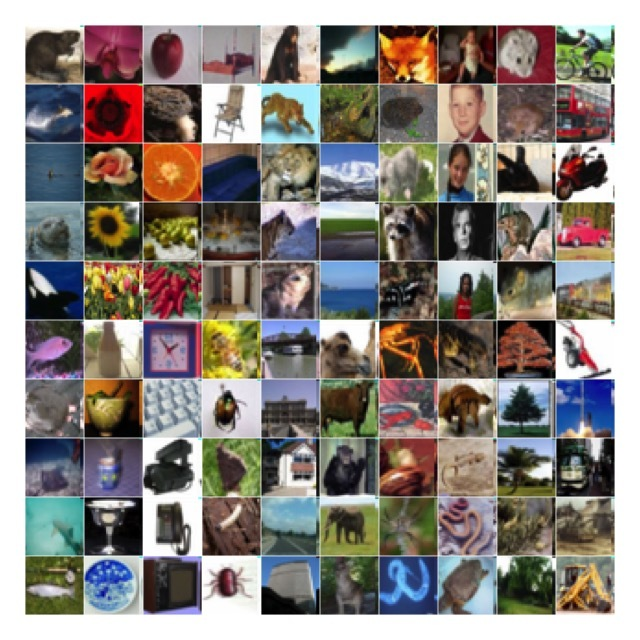
\includegraphics[width=0.5\textwidth]{images/cifar100}
\caption{An example set of images from CIFAR-100. From \cite{cifar100-sample}}
\label{fig:cifar100}
\end{figure}

A particular point of interest with CIFAR-100 is that there are relatively few images per class.
This means that it is a dataset for which overfitting is a critical concern.
Typical algorithms, without any specially designed methods, can often achieve around 60\% accuracy on the testing dataset.
This, however, tends to represent a hard limit.
Training accuracy will usually hit nearly 100\% accuracy, meaning that the network has learned all it can from the training dataset.
The difference between testing and training accuracy, especially with the limited data available, is the primary area of improvement for modern algorithms.

We perform a base experiment on a residual network with 30 residual blocks (60 layers), with channel sizes starting at 16 and increasing by a factor of 2 every 10 layers.
This structure was originally built for the ImageNet dataset.
However, we adapt it to CIFAR-100, which has much smaller images and therefore requires less capacity in the network.
Again utilizing common practice, we use minibatches of size 128, and sample training accuracy every 100 steps.
We allow training to proceed until error rates drop inperceptibly over a reasonably significant period of time.
We see the expected training accuracy go to 100\%, but the testing accuracy hovers around 65\%, which is also in line with expectations.

In our first experiment, we again use the same basic algorithm first developed for the sine experiment and let the network learn in tenths.
Observing the error rates from the static experiment, we let the network expand every 25 samples (representing 2500 steps).
This is an extremely restrictive network, and our results show that this is perhaps overconstrained for the problem; the training error peaks at 80\% while the testing error hovers around 58\%.
While this is a noticeably poorer result, it is still interesting to note that the generalization appears to be better in this experiment, as the difference between the training and testing error falls from 35\% to 22\%.
Even in the prior static baseline, there was never a comparably small difference between the training and testing error.
This leads us to consider how we can better understand the generalizability of our algorithm, which we discuss in the following chapter.

This performance is summarized in Figure~\ref{fig:cifar_accuracy}. % and Figure~\ref{fig:cifar_loss}.
We include results from our final experiment, which we discuss below.
Unfortunately, these results are based on the training loss and accuracy rather than testing accuracy, due to a few bugs in the software.
Nevertheless, we provide this figure to demonstrate the difficulties in optimizing the standard network, as the adaptive methods are unable to achieve the same results.
This also furthers our discussion on generalization.
While the training error does not decrease as significantly, we are still able to tune the algorithm to surpass the standard network in our second experiment.


\begin{figure}[!htb]
\centering
\resizebox{0.8\textwidth}{!}{% GNUPLOT: LaTeX picture with Postscript
\begingroup
  \makeatletter
  \providecommand\color[2][]{%
    \GenericError{(gnuplot) \space\space\space\@spaces}{%
      Package color not loaded in conjunction with
      terminal option `colourtext'%
    }{See the gnuplot documentation for explanation.%
    }{Either use 'blacktext' in gnuplot or load the package
      color.sty in LaTeX.}%
    \renewcommand\color[2][]{}%
  }%
  \providecommand\includegraphics[2][]{%
    \GenericError{(gnuplot) \space\space\space\@spaces}{%
      Package graphicx or graphics not loaded%
    }{See the gnuplot documentation for explanation.%
    }{The gnuplot epslatex terminal needs graphicx.sty or graphics.sty.}%
    \renewcommand\includegraphics[2][]{}%
  }%
  \providecommand\rotatebox[2]{#2}%
  \@ifundefined{ifGPcolor}{%
    \newif\ifGPcolor
    \GPcolorfalse
  }{}%
  \@ifundefined{ifGPblacktext}{%
    \newif\ifGPblacktext
    \GPblacktexttrue
  }{}%
  % define a \g@addto@macro without @ in the name:
  \let\gplgaddtomacro\g@addto@macro
  % define empty templates for all commands taking text:
  \gdef\gplbacktext{}%
  \gdef\gplfronttext{}%
  \makeatother
  \ifGPblacktext
    % no textcolor at all
    \def\colorrgb#1{}%
    \def\colorgray#1{}%
  \else
    % gray or color?
    \ifGPcolor
      \def\colorrgb#1{\color[rgb]{#1}}%
      \def\colorgray#1{\color[gray]{#1}}%
      \expandafter\def\csname LTw\endcsname{\color{white}}%
      \expandafter\def\csname LTb\endcsname{\color{black}}%
      \expandafter\def\csname LTa\endcsname{\color{black}}%
      \expandafter\def\csname LT0\endcsname{\color[rgb]{1,0,0}}%
      \expandafter\def\csname LT1\endcsname{\color[rgb]{0,1,0}}%
      \expandafter\def\csname LT2\endcsname{\color[rgb]{0,0,1}}%
      \expandafter\def\csname LT3\endcsname{\color[rgb]{1,0,1}}%
      \expandafter\def\csname LT4\endcsname{\color[rgb]{0,1,1}}%
      \expandafter\def\csname LT5\endcsname{\color[rgb]{1,1,0}}%
      \expandafter\def\csname LT6\endcsname{\color[rgb]{0,0,0}}%
      \expandafter\def\csname LT7\endcsname{\color[rgb]{1,0.3,0}}%
      \expandafter\def\csname LT8\endcsname{\color[rgb]{0.5,0.5,0.5}}%
    \else
      % gray
      \def\colorrgb#1{\color{black}}%
      \def\colorgray#1{\color[gray]{#1}}%
      \expandafter\def\csname LTw\endcsname{\color{white}}%
      \expandafter\def\csname LTb\endcsname{\color{black}}%
      \expandafter\def\csname LTa\endcsname{\color{black}}%
      \expandafter\def\csname LT0\endcsname{\color{black}}%
      \expandafter\def\csname LT1\endcsname{\color{black}}%
      \expandafter\def\csname LT2\endcsname{\color{black}}%
      \expandafter\def\csname LT3\endcsname{\color{black}}%
      \expandafter\def\csname LT4\endcsname{\color{black}}%
      \expandafter\def\csname LT5\endcsname{\color{black}}%
      \expandafter\def\csname LT6\endcsname{\color{black}}%
      \expandafter\def\csname LT7\endcsname{\color{black}}%
      \expandafter\def\csname LT8\endcsname{\color{black}}%
    \fi
  \fi
    \setlength{\unitlength}{0.0500bp}%
    \ifx\gptboxheight\undefined%
      \newlength{\gptboxheight}%
      \newlength{\gptboxwidth}%
      \newsavebox{\gptboxtext}%
    \fi%
    \setlength{\fboxrule}{0.5pt}%
    \setlength{\fboxsep}{1pt}%
\begin{picture}(7200.00,5040.00)%
    \gplgaddtomacro\gplbacktext{%
      \csname LTb\endcsname%
      \put(814,1275){\makebox(0,0)[r]{\strut{}$0$}}%
      \put(814,1568){\makebox(0,0)[r]{\strut{}$0.1$}}%
      \put(814,1861){\makebox(0,0)[r]{\strut{}$0.2$}}%
      \put(814,2154){\makebox(0,0)[r]{\strut{}$0.3$}}%
      \put(814,2447){\makebox(0,0)[r]{\strut{}$0.4$}}%
      \put(814,2740){\makebox(0,0)[r]{\strut{}$0.5$}}%
      \put(814,3032){\makebox(0,0)[r]{\strut{}$0.6$}}%
      \put(814,3325){\makebox(0,0)[r]{\strut{}$0.7$}}%
      \put(814,3618){\makebox(0,0)[r]{\strut{}$0.8$}}%
      \put(814,3911){\makebox(0,0)[r]{\strut{}$0.9$}}%
      \put(814,4204){\makebox(0,0)[r]{\strut{}$1$}}%
      \put(946,1055){\makebox(0,0){\strut{}$0$}}%
      \put(1922,1055){\makebox(0,0){\strut{}$200$}}%
      \put(2898,1055){\makebox(0,0){\strut{}$400$}}%
      \put(3875,1055){\makebox(0,0){\strut{}$600$}}%
      \put(4851,1055){\makebox(0,0){\strut{}$800$}}%
      \put(5827,1055){\makebox(0,0){\strut{}$1000$}}%
      \put(6803,1055){\makebox(0,0){\strut{}$1200$}}%
    }%
    \gplgaddtomacro\gplfronttext{%
      \csname LTb\endcsname%
      \put(176,2739){\rotatebox{-270}{\makebox(0,0){\strut{}accuracy}}}%
      \put(3874,725){\makebox(0,0){\strut{}epoch}}%
      \csname LTb\endcsname%
      \put(5816,4031){\makebox(0,0)[r]{\strut{}standard}}%
      \csname LTb\endcsname%
      \put(5816,3811){\makebox(0,0)[r]{\strut{}adaptive-1}}%
      \csname LTb\endcsname%
      \put(5816,3591){\makebox(0,0)[r]{\strut{}adaptive-2}}%
    }%
    \gplbacktext
    \put(0,0){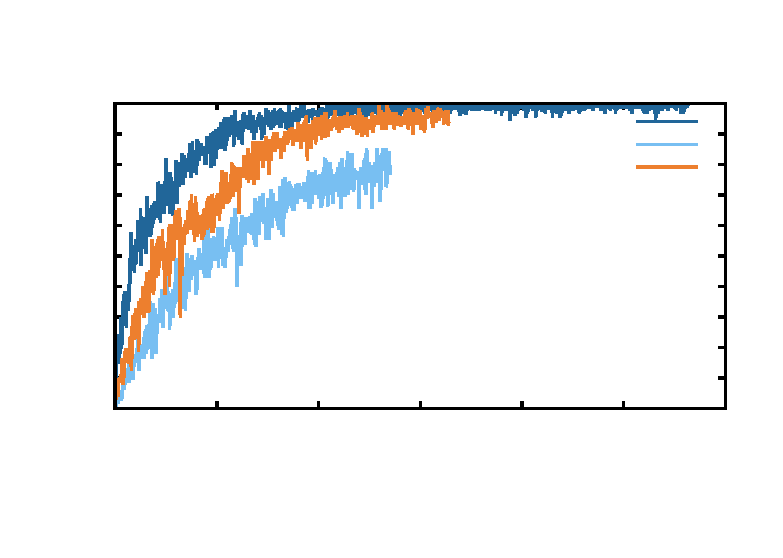
\includegraphics{cifar_accuracy}}%
    \gplfronttext
  \end{picture}%
\endgroup
}
\caption{CIFAR-100 training accuracy.}
\label{fig:cifar_accuracy}
\end{figure}

%\begin{figure}[!htb]
%\centering
%\resizebox{0.8\textwidth}{!}{% GNUPLOT: LaTeX picture with Postscript
\begingroup
  \makeatletter
  \providecommand\color[2][]{%
    \GenericError{(gnuplot) \space\space\space\@spaces}{%
      Package color not loaded in conjunction with
      terminal option `colourtext'%
    }{See the gnuplot documentation for explanation.%
    }{Either use 'blacktext' in gnuplot or load the package
      color.sty in LaTeX.}%
    \renewcommand\color[2][]{}%
  }%
  \providecommand\includegraphics[2][]{%
    \GenericError{(gnuplot) \space\space\space\@spaces}{%
      Package graphicx or graphics not loaded%
    }{See the gnuplot documentation for explanation.%
    }{The gnuplot epslatex terminal needs graphicx.sty or graphics.sty.}%
    \renewcommand\includegraphics[2][]{}%
  }%
  \providecommand\rotatebox[2]{#2}%
  \@ifundefined{ifGPcolor}{%
    \newif\ifGPcolor
    \GPcolorfalse
  }{}%
  \@ifundefined{ifGPblacktext}{%
    \newif\ifGPblacktext
    \GPblacktexttrue
  }{}%
  % define a \g@addto@macro without @ in the name:
  \let\gplgaddtomacro\g@addto@macro
  % define empty templates for all commands taking text:
  \gdef\gplbacktext{}%
  \gdef\gplfronttext{}%
  \makeatother
  \ifGPblacktext
    % no textcolor at all
    \def\colorrgb#1{}%
    \def\colorgray#1{}%
  \else
    % gray or color?
    \ifGPcolor
      \def\colorrgb#1{\color[rgb]{#1}}%
      \def\colorgray#1{\color[gray]{#1}}%
      \expandafter\def\csname LTw\endcsname{\color{white}}%
      \expandafter\def\csname LTb\endcsname{\color{black}}%
      \expandafter\def\csname LTa\endcsname{\color{black}}%
      \expandafter\def\csname LT0\endcsname{\color[rgb]{1,0,0}}%
      \expandafter\def\csname LT1\endcsname{\color[rgb]{0,1,0}}%
      \expandafter\def\csname LT2\endcsname{\color[rgb]{0,0,1}}%
      \expandafter\def\csname LT3\endcsname{\color[rgb]{1,0,1}}%
      \expandafter\def\csname LT4\endcsname{\color[rgb]{0,1,1}}%
      \expandafter\def\csname LT5\endcsname{\color[rgb]{1,1,0}}%
      \expandafter\def\csname LT6\endcsname{\color[rgb]{0,0,0}}%
      \expandafter\def\csname LT7\endcsname{\color[rgb]{1,0.3,0}}%
      \expandafter\def\csname LT8\endcsname{\color[rgb]{0.5,0.5,0.5}}%
    \else
      % gray
      \def\colorrgb#1{\color{black}}%
      \def\colorgray#1{\color[gray]{#1}}%
      \expandafter\def\csname LTw\endcsname{\color{white}}%
      \expandafter\def\csname LTb\endcsname{\color{black}}%
      \expandafter\def\csname LTa\endcsname{\color{black}}%
      \expandafter\def\csname LT0\endcsname{\color{black}}%
      \expandafter\def\csname LT1\endcsname{\color{black}}%
      \expandafter\def\csname LT2\endcsname{\color{black}}%
      \expandafter\def\csname LT3\endcsname{\color{black}}%
      \expandafter\def\csname LT4\endcsname{\color{black}}%
      \expandafter\def\csname LT5\endcsname{\color{black}}%
      \expandafter\def\csname LT6\endcsname{\color{black}}%
      \expandafter\def\csname LT7\endcsname{\color{black}}%
      \expandafter\def\csname LT8\endcsname{\color{black}}%
    \fi
  \fi
    \setlength{\unitlength}{0.0500bp}%
    \ifx\gptboxheight\undefined%
      \newlength{\gptboxheight}%
      \newlength{\gptboxwidth}%
      \newsavebox{\gptboxtext}%
    \fi%
    \setlength{\fboxrule}{0.5pt}%
    \setlength{\fboxsep}{1pt}%
\begin{picture}(7200.00,5040.00)%
    \gplgaddtomacro\gplbacktext{%
      \csname LTb\endcsname%
      \put(814,1275){\makebox(0,0)[r]{\strut{}$0$}}%
      \put(814,1568){\makebox(0,0)[r]{\strut{}$0.5$}}%
      \put(814,1861){\makebox(0,0)[r]{\strut{}$1$}}%
      \put(814,2154){\makebox(0,0)[r]{\strut{}$1.5$}}%
      \put(814,2447){\makebox(0,0)[r]{\strut{}$2$}}%
      \put(814,2740){\makebox(0,0)[r]{\strut{}$2.5$}}%
      \put(814,3032){\makebox(0,0)[r]{\strut{}$3$}}%
      \put(814,3325){\makebox(0,0)[r]{\strut{}$3.5$}}%
      \put(814,3618){\makebox(0,0)[r]{\strut{}$4$}}%
      \put(814,3911){\makebox(0,0)[r]{\strut{}$4.5$}}%
      \put(814,4204){\makebox(0,0)[r]{\strut{}$5$}}%
      \put(946,1055){\makebox(0,0){\strut{}$0$}}%
      \put(1922,1055){\makebox(0,0){\strut{}$200$}}%
      \put(2898,1055){\makebox(0,0){\strut{}$400$}}%
      \put(3875,1055){\makebox(0,0){\strut{}$600$}}%
      \put(4851,1055){\makebox(0,0){\strut{}$800$}}%
      \put(5827,1055){\makebox(0,0){\strut{}$1000$}}%
      \put(6803,1055){\makebox(0,0){\strut{}$1200$}}%
    }%
    \gplgaddtomacro\gplfronttext{%
      \csname LTb\endcsname%
      \put(176,2739){\rotatebox{-270}{\makebox(0,0){\strut{}loss}}}%
      \put(3874,725){\makebox(0,0){\strut{}epoch}}%
      \csname LTb\endcsname%
      \put(5816,4031){\makebox(0,0)[r]{\strut{}standard}}%
      \csname LTb\endcsname%
      \put(5816,3811){\makebox(0,0)[r]{\strut{}adaptive-1}}%
      \csname LTb\endcsname%
      \put(5816,3591){\makebox(0,0)[r]{\strut{}adaptive-2}}%
    }%
    \gplbacktext
    \put(0,0){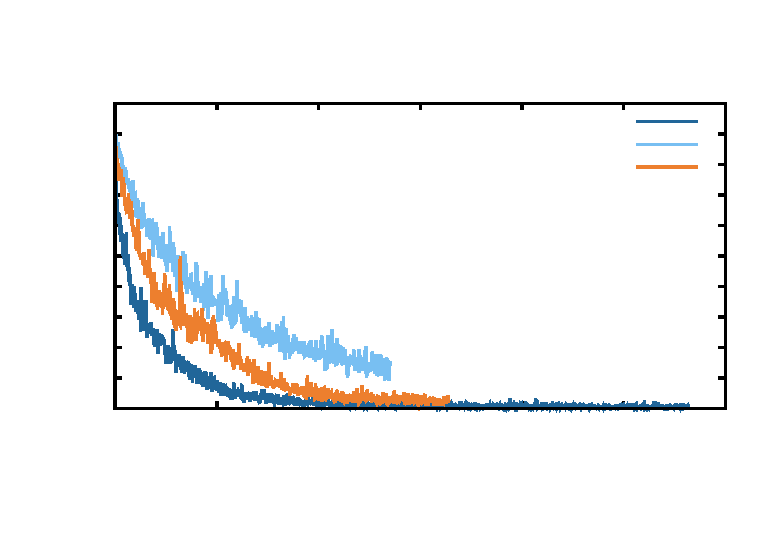
\includegraphics{cifar_loss}}%
    \gplfronttext
  \end{picture}%
\endgroup
}
%\caption{CIFAR-100 training loss.}
%\label{fig:cifar_loss}
%\end{figure}

We also note that that accuracy on the dataset is just one measure of precision.
During our experiments, we also log the cross-entropy loss, which provides a sense of not just how likely the network was to get the right answer, but how confidently it did so.
That is, while the accuracy is determined by picking the category with the highest activation, this choice may have been a very close decision.
For example, on a binary classification problem with classes 0 and 1, where the correct response is nearly always 1, a network with constant output activations $[0.49, 0.51]$ would have extremely low error but high cross-entropy loss.
Using this metric, we note that the cross-entropy loss is lower at the same training error for our methodology, indicating that its outputs are more regularized.

To improve the performance of this algorithm, we perform another experiment where we gradually allow a limited proportion (50\%) of the network to unfreeze over time.
We believe that this can be helpful in unlocking some of the limited capacity in the network; in particular, we note that the first few convolutional layers are fed into a very narrow pipeline of only 16 filters at full capacity.
Our training algorithm limits this further, which may overly constrict the flow of information through the network.
By leaving at least half of the capacity to be trained, we attempt to allow sufficient flow for better accuracy.
This hypothesis is borne out by the results, which show that the new network (entitled ``Adaptive-2'' in the figures) is able to demonstrate a small but significant improvement over the standard network.
We achieve a stable testing accuracy of 68\%, but interestingly, our training accuracy stabilizes at a lower point at around 95\%.
The results of our experiments are summarized in full in Table~\ref{table:cifar}.

\begin{table}[!htb]
\centering
\caption{CIFAR-100 results}
\label{table:cifar}
\begin{tabular}{@{}lrrr@{}}
\toprule
Network    & Testing Accuracy & Training Accuracy & Training Loss \\ \midrule
Standard   & 0.659            & 0.9927            & 0.0221        \\
Adaptive-1 & 0.582            & 0.8001            & 0.6595        \\
Adaptive-2 & 0.681            & 0.9557            & 0.1379        \\ \bottomrule
\end{tabular}
\end{table}


\section{Performance}
We note that our algorithm involves nearly no overhead over the original architecture; a simple timing benchmark over 1000 epochs of MNIST indicates a performance difference of 3.5\% (37.9 seconds versus 36.6 seconds), which is well within the margin of error.
Furthermore, by limiting the capacity of the network, we are able to achieve far faster initial training.
The initial timing experiment was performed by applying the algorithm but forcing it to use the full capacity of the network initially; this is far from the original intent.
By utilizing it in the same way as developed for the experiments, the first 1000 epochs of MNIST actually take 11.9 seconds, which is a huge improvement.
This performance boost can make a significant difference over the course of a training cycle.

While the algorithm takes more epochs to converge, the increased speed of working through the initial epochs is a significant boon.
In general, any decrease in performance can likely be attributed to the more intricate methods required to perform basic variable operations, recalling Listing~\ref{lst:var_deconst}.
These are generally considered to be minor; in fact, for most researchers, the choice of deep learning library is rarely made for performance reasons, especially for single-GPU servers.
Nearly all of the time spent is within the intricacies of the CUDNN module which interfaces directly with the GPU.
Our algorithm adds effectively no stress to the GPU, and can speed up training even when running at full capacity by fixing portions of the network, thus eliminating the need to perform the expensive gradient calculations.